\section{Graph Data Structures}
\label{section:12-Graph-Data-Structures}
\osullikomment{@REVIEWERS - START HERE FOR NOW}

\osullikomment{Add section overview}

% Graph-Based AI -- Include a discussion on the Overlap between Sybmolic (graph) and sub-symbolic (Generative) AI.
% \subsection{Notation}
% \label{section:121-graph-notation}

% %
% \nrscomment{Id put these in the style of the way math papers introduce notation. bolded Definition. type thing. You have it as prose currently, but its very choppy to read as prose, so you may as well lean into this being a bunch of definitions}
% %
% This section outlines the notation and terminology that will be used throughout the remainder of this thesis.
% A \textit{Graph}, sometimes called a \textit{Network} in the social sciences, is a foundational data structure and computing concept to describe combinatorial structures~\cite{Kleinberg2014}. 
% The simplest graph $G$ has two components. 
% The \textit{Vertices} $V$, sometimes called \textit{Nodes} is a set of objects that represent `entities' or `things'.
% The \textit{Edges} $E$, sometimes called \textit{Arcs} or \textit{Links} are the set of connections between the vertices that describe some relation between them.

% %
% \nrscomment{here seems like the better place to mention attributed edges. a bit jarring circling back to it down below after topology.}

% \nrscomment{youre also going from defining graph components to higher level graph features here. i dont think you finished with components (hyper edge? multi edge?) and a signal of the switch would help with navigating this section}
% %
% So, the graph $G$ has the sets of vertices ($V$) and edges ($E$), giving us $G = \{V,E\}$.
% The \textit{Degree} ($K$) of a vertex is the count of the edges it participates in. 
% In directed graphs, it is often separated to \textit{in-degree} ($K_{in}$) and \textit{out-degree} ($K_{out}$).
% The structure of the graph, the pattern formed by the vertices and edges that connect them is the \textit{topology} of the graph. 

% %
% \nrscomment{put the term before the defn i.e. the topology is...}
% %
% The \textit{topology} is the distinctive feature of a graph data structure.
% Analyzing and exploiting the \textit{topology} is core to many algorithms that seek to solve graph problems. 

% %
% \nrscomment{the defns below these seem kind of arbitrary, will you actually use them? are they relevant?}
% %
% The \textit{diameter} of the graph is the length of the shortest path between the two most `distant' nodes.
% The \textit{eccentricity} of a graph is the greatest geodesic distance between two vertices in the graph~\cite{Wu2015}.
% The \textit{radius} of the graph is the minimum graph eccentricity.~\cite{Wu2015}
% The \textit{algebraic connectivity} of a graph describes how well-connected it is~\cite{Wu2015}
% the \textit{traversal depth} of a graph algorithm is how many traverse iterations need to occur to complete an algorithm and is directly proportional to the eccentricity and connectivity of a graph~\cite{Wu2015}. 



% Figures~\ref{figure:graph-simple}--~\ref{figure:graph-multi} show how quickly complexity builds in graphs with the addition of attributes (labels), direction, weights and heterogeneous vertex and edge types.

% %
% \nrscomment{i'm not sure saying they show complexity is really what you want, maybe just that the fig shows the variety of basic properties a graph can have?}
% %


\osullikomment{Combine into subfigures}

%Rendering of the simplest possible Graph
\begin{figure}
    \begin{center}
        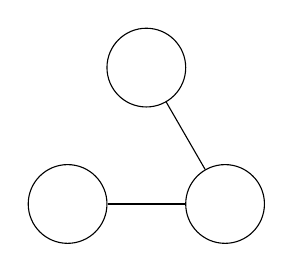
\begin{tikzpicture}
            % Define vertices
            \node[circle,draw,minimum size=1cm] (A) at (0,0) {};
            \node[circle,draw,minimum size=1cm] (B) at (2,0) {};
            \node[circle,draw,minimum size=1cm] (C) at (1,1.732) {};
            
            % Draw edges
            \draw (A) -- (B);
            \draw (B) -- (C);
            \end{tikzpicture}
        \caption{A simple graph with three vertices and two edges.}
        \label{Figure:graph-simple}          
    \end{center}
\end{figure}
\begin{figure}
    \begin{center}
        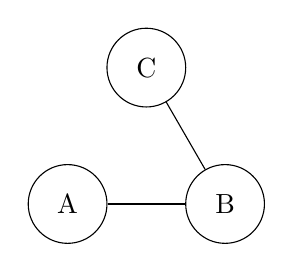
\begin{tikzpicture}
            % Define vertices
            \node[circle,draw,minimum size=1cm] (A) at (0,0) {A};
            \node[circle,draw,minimum size=1cm] (B) at (2,0) {B};
            \node[circle,draw,minimum size=1cm] (C) at (1,1.732) {C};
            
            % Draw edges
            \draw (A) -- (B);
            \draw (B) -- (C);
            \end{tikzpicture}
        \caption{A simple attributed graph with three named vertices and two edges.}
        \label{figure:graph-attributed}          
    \end{center}
\end{figure}
\begin{figure}
    \begin{center}
        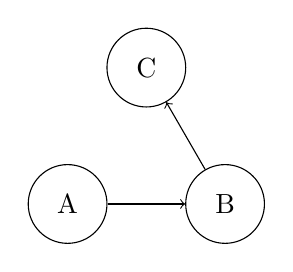
\begin{tikzpicture}
            % Define vertices
            \node[circle,draw,minimum size=1cm] (A) at (0,0) {A};
            \node[circle,draw,minimum size=1cm] (B) at (2,0) {B};
            \node[circle,draw,minimum size=1cm] (C) at (1,1.732) {C};
            
            % Draw edges
            \draw[->](A) -- (B);
            \draw[->](B) -- (C);
            \end{tikzpicture}
        \caption{A simple attributed graph with three named vertices and two directed edges.}
        \label{Figure:graph-directed}          
    \end{center}
\end{figure}
\begin{figure}
    \begin{center}
        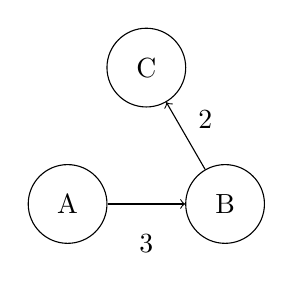
\begin{tikzpicture}            
            % Define vertices
            \node[circle,draw,minimum size=1cm] (A) at (0,0) {A};
            \node[circle,draw,minimum size=1cm] (B) at (2,0) {B};
            \node[circle,draw,minimum size=1cm] (C) at (1,1.732) {C};
            \node at (1, -0.5) {3};
            \node at (1.75, 1.075) {2};
            
            % Draw edges
            \draw[->](A) -- (B);
            \draw[->](B) -- (C);
            \end{tikzpicture}
        \caption{A simple attributed graph with three named vertices and two directed weighted edges.}
        \label{figure:graph-weighted}          
    \end{center}
\end{figure}
\begin{figure}
    \begin{center}
        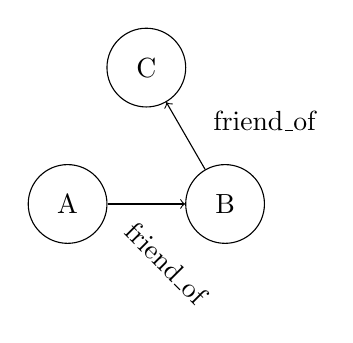
\begin{tikzpicture}            
            % Define vertices
            \node[circle,draw,minimum size=1cm] (A) at (0,0) {A};
            \node[circle,draw,minimum size=1cm] (B) at (2,0) {B};
            \node[circle,draw,minimum size=1cm] (C) at (1,1.732) {C};
            \node at (1.25, -0.75) {\rotatebox{-45}{friend\_of}};
            \node at (2.5, 1.05) {friend\_of};
            
            % Draw edges
            \draw[->](A) -- (B);
            \draw[->](B) -- (C);
            \end{tikzpicture}
        \caption{A simple attributed graph with three named vertices and two directed labeled edges.}
        \label{figure:graph-labeled}          
    \end{center}
\end{figure}
\begin{figure}
    \begin{center}
        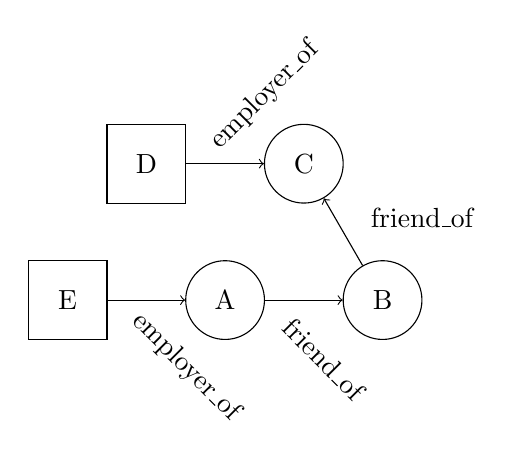
\begin{tikzpicture}            
            % Define vertices
            \node[circle,draw,minimum size=1cm] (A) at (0,0) {A};
            \node[circle,draw,minimum size=1cm] (B) at (2,0) {B};
            \node[circle,draw,minimum size=1cm] (C) at (1,1.732) {C};
            \node[rectangle,draw,minimum size=1cm] (D) at (-1,1.732) {D};
            \node[rectangle,draw,minimum size=1cm] (E) at (-2,0) {E};
            \node at (1.25, -0.75) {\rotatebox{-45}{friend\_of}};
            \node at (2.5, 1.05) {friend\_of};
            \node at (-0.5, -0.85) {\rotatebox{-45}{employer\_of}};
            \node at (0.5, 2.6) {\rotatebox{45}{employer\_of}};
            
            % Draw edges
            \draw[->](A) -- (B);
            \draw[->](B) -- (C);
            \draw[->](D) -- (C);
            \draw[->](E) -- (A);
            \end{tikzpicture}
        \caption{A heterogeneous directed attributed graph with three `employee' vertices and two `company' vertices. A very simple knowledge graph.}
        \label{figure:graph-heterogeneous}          
    \end{center}
\end{figure}
\begin{figure}
    \begin{center}
        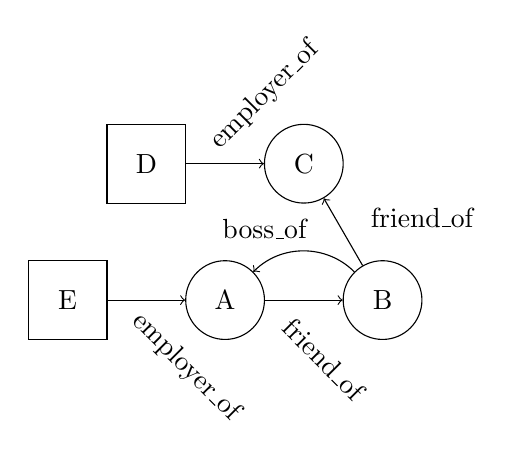
\begin{tikzpicture}            
            % Define vertices
            \node[circle,draw,minimum size=1cm] (A) at (0,0) {A};
            \node[circle,draw,minimum size=1cm] (B) at (2,0) {B};
            \node[circle,draw,minimum size=1cm] (C) at (1,1.732) {C};
            \node[rectangle,draw,minimum size=1cm] (D) at (-1,1.732) {D};
            \node[rectangle,draw,minimum size=1cm] (E) at (-2,0) {E};
            \node at (1.25, -0.75) {\rotatebox{-45}{friend\_of}};
            \node at (2.5, 1.05) {friend\_of};
            \node at (-0.5, -0.85) {\rotatebox{-45}{employer\_of}};
            \node at (0.5, 2.6) {\rotatebox{45}{employer\_of}};
            \node at (0.5, 0.9) {boss\_of};
            
            % Draw edges
            \draw[->](A) -- (B);
            \draw[->](B) -- (C);
            \draw[->](D) -- (C);
            \draw[->](E) -- (A);
            \draw [->] (B) to [out=135,in=45] (A);
            \end{tikzpicture}
        \caption{A heterogeneous directed attributed multi-graph with three `employee' vertices and two `company' vertices. Multiple different types of edges can exist between nodes of the same type. A very simple knowledge graph.}
        \label{Figure:graph-multi}          
    \end{center}
\end{figure}

\subsection{Graph Representation}
\label{section:122-graph-representation}

% %
% \nrscomment{again here some more structure than a block of prose might help the reader refer back to the different representations later, esp since youre giving the same kind of info for each (space complexity, etc.) maybe summarize in a table as well?}
% %

% Graphs can be represented in numerous ways, with the two most common being the \textit{Adjacency List} and \textit{Adjacency Matrix} formats. 
% Consider the graph in figure~\ref{figure:graph-example} with five vertices and five edges.
% Representing it using an adjacency list (figure~\ref{figure:graph-adj-list}) yields a small memory footprint ($\mathcal{O}(|V|+|E|)$), but finding a particular edge is expensive being linear in the number of vertices ($\mathcal{O}(|V|)$) in the worst case.
% Conversely, representing it as an \textit{adjacency matrix} (figure~\ref{figure:adjacency_matrix}) has a memory footprint of $\mathcal{O}(|V|^{2})$ but a constant lookup time ($\mathcal{O}(1)$).
% The tradeoff between memory efficiency and lookup efficiency is a core tension in graph processing and many of the attempts to accelerate the efficiency of graph algorithms focus on balancing these two dimensions (see section~\ref{section:13-Graph-Hardware-Acceleration}).

% %
% \nrscomment{the sentence about the tradeoff i think ought to be your opener for this subsection. tucked in after the first two representations is too late- i need to know why i even care about representation in the first place before im willing to read it}
% %

% The adjacency list and adjacency matrix are capable of implicitly encoding the direction of edges but are not innately capable of representing edge weights or multigraph structures. 
% \nrscomment{para sep ought to be here instead}
% Another encoding of graphs, the \textit{incidence matrix}, encodes both the source and destination of an edge. 
% The representation in figure~\ref{figure:incidence_matrix} uses a negative integer to indicate the source, and a positive to indicate the destination. 
% The integers can be replaced with any real number to represent weights, encoding more information.
% Because the edges are represented as distinct entities, the \textit{incidence matrix} is capable of representing more complicated graph formats that are directed, weighted, multi-edge and hyper-edge~\cite{Kepner2016}.
% % %
% % \nrscomment{i dont think youve defined multi/hyper edge, have you?}
% % %


% %
% \nrscomment{youre using |.| to mean cardinality, i think, so it might be worth writing that out in words as well as reminding what V, E are, i.e. the space complexity is O(...), where |V| represents the number of vertices and |E| represents the number of edges}
% %
% The space complexity of an incidence matrix is $\mathcal{O}(|V|\times|E|)$ and so for sparse graphs may be more space-efficient than an \textit{adjacency matrix} but in general will consume more memory where $|E|>|V|$.

% %
% \nrscomment{again maybe worth writing out "... more memory when the number of edges is greater than the number of nodes, i.e. |E| > |V|"}
% %
% The lookup time for edge existence in an incidence matrix is also slower than for an adjacency list. 
% To find an edge connecting two vertices, we need to scan the entire edge list for each vertex and locate which edge(s), if any, are incident to both vertices, reducing to a complexity of $\mathcal{O}(|E|)$.

% Many formats have been developed to improve the balance between storage efficiency and lookup speed. 
% The dominant choices are the Compressed Sparse Row (CSR) and Compressed Sparse Column (CSC) formats.
% The CSR format uses three lists to compress the rows of a sparse matrix, like an adjacency matrix~\cite{Bulucc2009}. 
% First, the \textit{value list} contains every nonzero value of the matrix (the existence of an edge), and so has a length of $|E|$ in a directed adjacency matrix. 
% The \textit{Row Pointer} list contains the index of each position in the \textit{value list} that is associated with a new row.
% The \textit{Column Indices} list contains the column index of each value in the \textit{value list} from the original sparse matrix.
% So in figure~\ref{figure:csr}, the values associated with the \textbf{A} vertex (row $0$ of the adjacency matrix) are at positions $[0,1]$ in the value list in figure~\ref{figure:csr}. 
% We derive this by looking at the row index in figure~\ref{figure:csr} and seeing that the second row begins from index $2$.
% Knowing that the first two values in the value list are the sources of our edges, we know that the first two values in the column index in figure~\ref{figure:csr} are the destinations $[1,2]$.
% In the adjacency matrix (figure~\ref{figure:adjacency_matrix}), column $1$ is for vertex \textbf{B} and column $2$ is for vertex \textbf{C}. 

% %
% \nrscomment{what is your convention for bold/italics/emph? seems like italics for defns, bold for node variable names? Ive usually seen bold for definitions and italics for variable names}
% %

% The CSC format reverses the function of the row and column indices so that the columns are compressed.
% The space efficiency for CSR/CSC format is $\mathcal{O}(|V|\log(nnz)+nnz\log(|V|))$ for an adjacency matrix of $|V|$ vertices~\cite{Bulucc2009} and takes $\mathcal{O}(\log(nnz))$ time to check the existence of an edge where $nnz$ is the count of non zero entries in the matrix.

% % \begin{figure}
    \begin{center}
        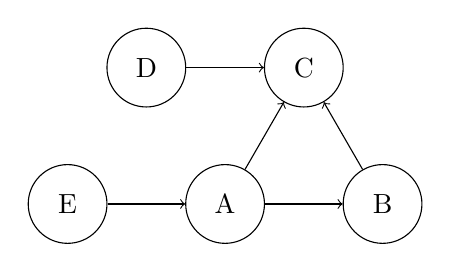
\begin{tikzpicture}
            % Define vertices
            \node[circle,draw,minimum size=1cm] (A) at (0,0) {A};
            \node[circle,draw,minimum size=1cm] (B) at (2,0) {B};
            \node[circle,draw,minimum size=1cm] (C) at (1,1.732) {C};
            \node[circle,draw,minimum size=1cm] (D) at (-1,1.732) {D};
            \node[circle,draw,minimum size=1cm] (E) at (-2,0) {E};
            
            % Draw edges
            \draw[->](A) -- (B);
            \draw[->](B) -- (C);
            \draw[->](D) -- (C);
            \draw[->](E) -- (A);
            \draw[->](A) -- (C);
            \end{tikzpicture}
        \caption{Example graph with five nodes and five edges}
        \label{figure:graph-example}          
    \end{center}
\end{figure}
% % 
\begin{figure}[h]
    \centering
    \begin{tikzpicture}[scale=1.5]
        \tikzstyle{vertex}=[circle,fill=black!25,minimum size=17pt,inner sep=0pt]
        \tikzstyle{edge} = [draw,thick,-]

        \matrix[matrix of math nodes,
          %left delimiter={[},
          %right delimiter={]},
          %below = 1cm of A,
          nodes={minimum width=3em, minimum height=3em, outer sep=0pt},
          column sep=-\pgflinewidth,
          row sep=-\pgflinewidth] (m) { A, & B, & C \\
                                        B, & C, &   \\
                                        C, &    &   \\
                                        D, & C, &   \\
                                        E, & A, &   \\
                                    };

    \end{tikzpicture}
    \caption{Adjacency List for graph in figure~\ref{figure:graph-example}. Each line represents a vertex with the first in the list being the source and each subsequent vertex a destination of an edge.}
    \label{figure:graph-adj-list}
\end{figure}

% % 
\begin{figure}[h]
\centering
\begin{tikzpicture}[>=stealth, shorten >=1pt, auto, node distance=3cm, thick, main node/.style={circle, draw, font=\sffamily\Large\bfseries}]

  % Render the adjacency matrix
  \matrix[matrix of math nodes,
          left delimiter={[},
          right delimiter={]},
          %below = 1cm of A,
          nodes={minimum width=3em, minimum height=3em, outer sep=0pt},
          column sep=-\pgflinewidth,
          row sep=-\pgflinewidth] (m) {   & A & B & C & D & E \\
                                        A & 0 & 1 & 1 & 0 & 0 \\
                                        B & 0 & 0 & 1 & 0 & 0 \\
                                        C & 0 & 0 & 0 & 0 & 0 \\
                                        D & 0 & 0 & 1 & 0 & 0 \\
                                        E & 1 & 0 & 0 & 0 & 0 \\
                                    };

\end{tikzpicture}
\caption{Adjacency Matrix for graph in Figure~\ref{Figure:graph-example} is a $|V| \times |V|$ matrix where a value of $1$ indicates an edge and $0$ is no edge.}
\label{Figure:adjacency_matrix}
\end{figure}

% % 
\begin{figure}[h]
    \centering
    \begin{tikzpicture}[>=stealth, shorten >=1pt, auto, node distance=3cm, thick, main node/.style={circle, draw, font=\sffamily\Large\bfseries}]
    
      % Render the adjacency matrix
      \matrix[matrix of math nodes,
                left delimiter={[},
                right delimiter={]},
                %below = 1cm of A,
                nodes={minimum width=3em, minimum height=3em, outer sep=0pt},
                column sep=-\pgflinewidth,
                row sep=-\pgflinewidth] (m) {   & e_0 & e_1 & e_2 & e_3 & e_4\\ 
                                            A   &  -1 &   0 &   0 &   1 &  -1\\
                                            B   &   1 &  -1 &   0 &   0 &   0\\
                                            C   &   0 &   1 &   1 &   0 &   1\\
                                            D   &   0 &   0 &  -1 &   0 &   0\\
                                            E   &   0 &   0 &   0 &  -1 &   1\\
                                            };
    
    \end{tikzpicture}
    \caption{Incidence Matrix for the graph in Figure~\ref{figure:graph-example} is a $|E| \times |V|$ matrix where a -1 is the source node and 1 is the destination of a given edge.}
    \label{figure:incidence_matrix}
    \end{figure}
    



% % \begin{figure}[h]
    \centering
    \begin{tikzpicture}[>=stealth, shorten >=1pt, auto, node distance=3cm, thick, main node/.style={circle, draw, font=\sffamily\Large\bfseries}]
    
      % Render the adjacency matrix
        \matrix[matrix of math nodes,
              left delimiter={[},
              right delimiter={]},
              %below = 1cm of A,
              nodes={minimum width=3em, minimum height=3em, outer sep=0pt},
              column sep=-\pgflinewidth,
              row sep=-\pgflinewidth] (M1) { 
                                            1 & 1 & 1 & 1 & 1 &\\
                                            };
        \node[left] at (M1.west) {Value List..};                                    
    \end{tikzpicture}

    \begin{tikzpicture}[>=stealth, shorten >=1pt, auto, node distance=3cm, thick, main node/.style={circle, draw, font=\sffamily\Large\bfseries}]

        \matrix[matrix of math nodes,
              left delimiter={[},
              right delimiter={]},
            %below = M1,
              nodes={minimum width=3em, minimum height=3em, outer sep=0pt},
              column sep=-\pgflinewidth,
              row sep=-\pgflinewidth] (M2) { 
                                            0 & 2 & 2 & 3 & 4 & 5\\
                                            };
        \node[left] at (M2.west) {Row Index.............}; 
    \end{tikzpicture}

    \begin{tikzpicture}[>=stealth, shorten >=1pt, auto, node distance=3cm, thick, main node/.style={circle, draw, font=\sffamily\Large\bfseries}]

        \matrix[matrix of math nodes,
              left delimiter={[},
              right delimiter={]},
              %below = M2,
              nodes={minimum width=3em, minimum height=3em, outer sep=0pt},
              column sep=-\pgflinewidth,
              row sep=-\pgflinewidth] (M3) { 
                                            1 & 2 & 2 & 2 & 0 & \\
                                            };
        \node[left] at (M3.west) {Col Index...};
    
    \end{tikzpicture}
    \caption{The \ac{CSR} format uses three lists to represent the graph in Figure~\ref{Figure:graph-example}.}
    \label{Figure:csr}
    \end{figure}

% More complicated representations exist which are capable of compressing the graph representations even further. 
% \textit{Ligra+} uses an encoding scheme that splits the graph into two arrays \textit{Compressed Edges-in} and \textit{Compressed Edges-out}.
% The arrays use k-bit block encoding to approximately halve the memory requirements to represent each graph compared to CSC/CSR. 
% The compression has an encode/decode overhead that makes it impractical in serial systems but has been shown to improve overall performance in parallel implementations~\cite{Shun2015}.


% %
% \nrscomment{this is back to definitional, not representational, shouldnt it be in the previous subsection?}
% %
% Graphs can be \textit{Static} or \textit{Dynamic}.
% Static graphs are those that are pre-built and unchanging. 
% Algorithms can assume unlimited time to find a solution and that the representation itself will remain unchanged. 
% A \textit{Dynamic} graph (also called a \textit{streaming} graph is constructed on the fly, with vertices and edges being created, read, updated and deleted (CRUD) while graph analysis is occurring.

%
% \nrscomment{do i know what graph analysis is yet? this is a bit jarring}
% %
% The I\&S community is constantly collecting and removing data, and so must be able to operate on graphs in time-constrained settings between when information is added and when it is removed~\cite{Regli2022a}.
% %
% \nrscomment{why are we talking about use case stuff in definitions section? if theres a takeaway to this point then give it the explanation it needs, otherwise i dont really gain anything and it just seems like a random fact dropped in}
% %

% \osullikomment{Summary of Representation here}


% \subsection{Graph Primitives}
% \label{section:123-graph-primitives}
% \osullikomment{The back half of the primitives section is just points I collected in my travels and need to synthesize}
% \nrscomment{i think this primitives section should be a table, and then you A. explain why primitives matter then B. summarize the table and the key takeaway about how the primitives differ by representation format and there arent agreed-upon ones across all formats then C. why is that problematic}

% %
% \nrscomment{missing the opening sentence where you tell me what this section is and why i should care. what even is a primative? need that before i learn there's disagreement}

% \nrscomment{Suggest opening this with an example of a field with clear primatives and what they are, and then explain why graphs doesn't have that. Otherwise youre just listing things that could kind of be primatives but I have nothing to ground that to really appreciate the point youre trying to make}
% %
% There is no real agreement on what the building blocks of graph processing should be~\cite{Satish2014}.

% %
% \nrscomment{this bit about canonical representations is confusing and feels like its presented backwards. first tell me what a canonical representation is "canonical representation is the common ... something". then tell me about the memory thing. then tell me all those formats can be used for canonical representations. in fact, why is this in this section and not the intro to representations before you list them out and define them?}
% %
% The \textit{adjacency list, adjacency matrix, incidence matrix} and \textit{CSC/CSR} formats are all used for \textit{canonical} representations of graphs. 
% The \textit{canonical} representation of a graph views the vertices as a chunk of memory, and the edges as pointers between those chunks. 

% %
% \nrscomment{ok, i now think you might just need a subsubsection on how graphs can be stored. jamming spatial locality into here is unexpected and breaks up the flow}
% %
% These chunks may also include details of the labels, weights and other non-topological information stored in the graph, or just house pointers to that information.
% Using this representation for large and dense graphs causes the `chunks' of memory for neighboring nodes to not be spatially co-located. 
% Without spatial locality, modern processor optimizations like caching and prefetching are ineffective, and the processor will need to wait for the relevant node vertex to be retrieved from the main memory before continuing. 
% %
% \nrscomment{so what? i think this is probably important, but here isnt the place to talk about it, its a takeaway, or a motivation, or something, but it doesnt belong in "laying the groundwork and defining what you need to know to understand my thesis" section}
% %



% \osullikomment{Add in Combinatorial BLAS here. }
% Drawing inspiration from the relationship between the Basic Linear Algebra Subprogram (BLAS) library and the development of accelerators for Floating Point Operations (FLOPs), an alternative linear algebraic representation of graphs and implementation of graph algorithms is emerging. 
% The GraphBLAS project is an effort to formalize graph operations using linear algebra~\cite{Mattson2013}.
% Using the incidence matrices for graphs in a CSC/CSR format, the GrahBLAS is building a mathematical abstraction layer for graph operations based on the realization that graph operations are matrix operations~\cite{Kepner2015, Kepner2016}.
% %
% \nrscomment{that was too deep in the weeds- i was expecting to learn what graph primitives are and i got "theres this new project trying to abstract something". i think you may be able to cut that chunk altogether, unless it comes back to be important}
% %

% The GraphBLAS team identified five primitive operations and five additional compound operations that can be composed of primitive operations. 
% The five primitive operations are \textit{Construct Matrix from Triples (\textbf{Sparse}}), \textit{Extract Triples from a Matrix (\textbf{Find}}), \textit{Element-Wise addition (\textbf{SpEWiseA}}), \textit{Element-Wise Multiplication (\textbf{SpEWiseX}}), and \textit{Matrix Products (\textbf{SpGEMM}})~\cite{Kepner2015}.
% These primitive operations are composed to represent graph operations, like a single step in a Breadth First Search (BFS) which is a matrix-vector multiplication of the adjacency matrix and the vector representing the node(s) to start from~\cite{Kepner2016}.

% \osullikomment{Here down is 'collection of things I should probably include but haven't integrated yet' Lots of it is redundant and covered later. }

% Wu et al identify two families of graph primitive operation, \textit{traversal}-based and \textit{dense-computation}-based.
% Traversal-based primitives systematically explore neighbors until some condition is met and only deal with small subsets of vertices. 
% Dense-computation primitives expect most or all vertices to be active. 
% Traversal primitives include BFS, Betweenness-Centrality (BC), Single-Source Shortest Path (SSSP) and depending on implemenation Connected Components (CC)~\cite{Wu2015}.
% Dense-computation primitives include PageRank~\cite{Wu2015}.
% Ham includes \textit{Collaborative Filtering} as a dense-computation primitive~\cite{Ham2016}.
% Each of these `primitives' is an algorithm in its own right, and are commonly thought of as \textit{kernels} rather than a `primitive' operation.

% Some programming models offer more conceptual primitives. 
% GPU-based programming models utilize the Bulk-Synchronous Parallel (BSP) programming model. 
% The \textit{Gather-Apply-Scatter} (GAS) is a BSP approach that decomposes a graph program into the \textit{gather} phase which accumulates information about all the adjacent vertices. 
% The \textit{Apply} phase creates a new attribute on the active vertex with the computed results of the accumulated values from the previous step. 
% The \textit{Scatter} phase propagates a predicate evaluation on all adjacent edges and vertices~\cite{Wu2015}.
% The \textit{Data-Centric Model} (DCM) uses the \textit{Advance, Filter} and \textit{Compute} operations to manipulate the \textit{frontier} of vertices. 
% The \textit{frontier} is the collection of vertices currently `active' in the algorithm.
% The \textit{Advance} operation generates a new frontier by expanding the neighbors of the current vertex frontier. 
% the \textit{Filter} operation chooses a subset of the frontier based on some specified criteria.
% the \textit{Compute} operation executes some specified action on all vertices in the frontier~\cite{Wu2015}. 

% Several fundamental graph algorithms cannot be expressed as frontier-based algorithms.~\cite{Dhulipala2017}

% The Pegasus graph analysis system also takes a linear-algebraic view. 
% It introduces the \textit{Generalized Integrated Matrix-Vector Multiplication} (GIM-V), a generalization of standard matrix-vector multiplication.
% They decompose it into three atomic operations \textit{combine2, combineAll} and \textit{Apply}.
% They use these three operations to implement \textit{PageRank, Random Walk, Diamater Estimation} and \textit{Connected Components}.

% There are two families of Programming Models for Graphs. 
% \textit{Vertex-Centric} and \textit{Edge-Centric}.
% \textit{Vertex-Centric} models effectively express the entire algorithm as operations on a single vertex and its edges~\cite{Ham2016}
% \textit{Vertex-Centric} models have two functions \textit{vertex\_scatter} and \textit{vertex\_gather}.
% \textit{Vertex\_scatter} defines what operations need to be performed on a vertex, and \textit{vertex\_gather} applies that operation and updates the vertex. 
% The \textit{Edge-Centric} model has two functions \textit{edge\_scatter} and \textit{edge\_gather}.
% \textit{Edge\_scatter} sends the information of the source vertex and edge to the destination vertex where the \textit{edge\_gather} function applies the updates~\cite{Liu2019}. 

% The \textit{Single Instruction Multiple Data - X}  (SIMD-X) paradigm defines \textit{Active, Compute} and \textit{Combining} operations. Is a BSP paradigm that aims to extend beyond vertex or edge centric computing. 
% The \textit{Active} function filters the graph and returns only the vertices which meet the conditions to be `active'.
% The \textit{Compute} function defines the computation that happens on each edge. 
% \textit{Combine} merges all the computed updates. 

% The `canonical' representations do not appear to have clearly defined primitive operations in the general sense, though high-performance parallel processing programming paradigms have done significant work in this area~\cite{Dhulipala2021}.


%
% \nrscomment{below is the "why am i talking about primitives" bit, which should come at the start of the subsubsection, not the end}
% %
% The reasons that distilling primitive operations is important in benchmark design are, first, that identifying the primitives allows us to design micro-benchmarks to understand how each building block of an algorithm can be optimized. 
% Second, by limiting to a set of primitives, the hardware implementation of those primitives can be optimized, meaning that the hardware designers can focus on developing hardware for a few specific operations, rather than general-purpose ones. 

% %
% \nrscomment{i think you should cut 1.2.4 entirely}
% %

% \subsection{General Characteristics}
% \label{section:124-general-characteristics}
% \nrscomment{this section feels like it should be moved to the abstract graph benchmark design. these are basically your characteristics to vary and account for. it doesnt belong up here. rest of the comment sin this section still apply but assume that this whole chunk will be with the benchmark stuff later.}

% Decades of research yield the characteristics of graphs that are `generally true' and interact with the \textit{efficiency} of graph analytics.
% These graph characteristics focus on the \textit{topological} features of graphs.
% Depending on the context, the addition of attribute information may simplify or complicate the algorithms that operate on the graphs. 

% \textbf{Input dependence.} 
% %
% \nrscomment{"Input dependence" is not a graph characteristic, and this subsubsection talks about random graphs. I think you can just cut this chunk entirely, or maybe reframe it, since you keep bringing up random graphs when explaining the subsequent characteristics. Maybe you first describe broad classes of graph domains (synthetic vs real. then within that the hierarchy you drew out) and compare the 'naive' random graph that one might use for a benchmark to the others and highlight the characteristics that matter for the benchmark. For instance show random edges vs fully connected, visually, and then explain why it affects processing. And then repeat for the other characteristics.}
% %
% The \textit{efficiency} and \textit{effectiveness} of every graph algorithm depends on the size and shape of the input graph.
% The data dependence of graph algorithms is one of the driving reasons that empirical evaluation favors a collection of `real-world' graphs drawn from the domain of intended use.
% While the shapes of graphs exist on a spectrum, common `classes' of graphs exist. 
% %
% \nrscomment{ok, in that case you need a section explicitly outlining those classes, and possibly 
% a table comparing them across the characteristics you're about to describe. you currently have it mixed in with the characteristics, so i come away not understanding what the classes are or what the characteristics are. decouple them.}
% %
% \textit{Random Graphs} are the baseline. 
% A random graph is synthetic.
% It is generated by creating a set of vertices and then creating an edge between each vertex in the set with a given probability. 
% Formally, given $G(n,p)$ where $n$ is the number of vertices to create and $p$ is the probability of any two vertices being connected by an edge, the generator creates $n$ vertices $\{v \in V\}$, and the set of edges $E = \{(u,v)|u,v \in V, u \neq v$ with probability $P$\} yielding the random graph $G=\{V, E\}$~\cite{Erdhos1960}.
% Random graphs are important as they provide the point of reference for other graph characteristics, discussed below. 

% \textbf{Size Matters.}
% %
% \nrscomment{please a different header}
% \nrscomment{replace this entire description with a picture. this can be 2 sentences}
% %
% Section~\ref{section:11-Intelligence-Security-Context} identifies that graphs in the I\&S domain can be billions to trillions of vertices and edges. 
% The \textit{size} of a graph impacts graph processing. 
% In the most obvious sense, like all computations, there is some relationship between the size of the input and the time required to process it.
% The count of the vertices can give us a false understanding of the scale of the graph. 
% For example, suppose a graph with $10$ vertices. 
% Each vertex except for the first and last is connected by an undirected edge to only two other vertices, such that they form a straight line of $10$ vertices.
% The graph will have $10$ vertices and $9$ edges. 
% But, suppose a fully connected graph, where each of those vertices is connected to every other vertex.
% That then becomes a graph of $10$ vertices and $45$ edges.
% If directed (and symmetric), we would have $18$ and $90$ edges respectively for the same graph of $10$ vertices. 
% If it is a more complicated multi-graph structure the edge count could increase even further. 
% So, any discussion of graph `size' must also account for the number of edges. 
% \osullikomment{Needs a Cite}

% \textbf{Degree Distribution.}
% The \textit{size} of the graph is closely linked to the number of edges in it. 
% Beyond a raw edge count, consideration must be given to the Degree $K$, the mean degree $\bar{K}$, the mean in-degree $\bar{K}_{in}$ and mean out-degree $\bar{K}_{out}$ and the \textit{distribution} of these values across the graph. 
% %
% \nrscomment{we dont know what any of those things mean, or why 'consideration must be given' to them}
% %
% Random graphs are quite regular in their distribution of degrees, and we expect the modal degree to approximate the mean degree.
% Similarly, on graphs derived from physical phenomena like road networks, the mean degree is generally consistent.
% Conversely, graphs derived from social interactions like phone call records or follower lists on social media tend to follow a power-law distribution. 
% %
% \nrscomment{if youre going to define scale-free, do it properly}
% %
% In these \textit {`Scale-Free'} graphs only a small percentage of the vertices possess most of the edges, and most vertices have very few edges.
% Intuitively, consider that a few celebrities are extremely popular and have large followings, while most people have only small followings.
% The scale-free graph shape is one of the key drivers of computational \textit{inefficeny} in graph processing. (see: section~\ref{section:126-processing-bottlenecks}).
% \osullikomment{Needs a Cite}

% \textbf{Graph Diameter and Transitivity}
% The \textit{diameter} of the graph is the length of the shortest path between the two most `distant' nodes.
% The \textit{transitivity} describes the probability that adjacent nodes in a graph are connected. 
% The \textit{clustering coefficient} is a measure of the transitivity at a local or global level (with slightly different calculations depending on scope).

% Random graphs tend to have a middling diameter and clustering coefficient, depending on the density parameter used to generate the graph.
% Graphs derived from physical phenomena like road networks tend to have a large diameter and small global clustering coefficient.
% Scale-free graphs representing social phenomena like social media follower graphs tend to have a small diameter and large clustering coefficient. 
% Known as the \textit{small-world} characteristic, we can say that of a scale-free graph, most vertices are `close' to each other.
% Some graphs have a \textit{small-world} property in some component subgraphs but have other subgraphs that are of a larger diameter and lower density.

% The variance in the diameter and density of graphs, even internally on large complicated graphs like \textit{knowledge graphs} means that a graph processing algorithm may need to intermittently deal with extremely dense and sparse sections within the same algorithm, complicating the ability to efficiently process them.
% \osullikomment{Needs a Cite}


% \textbf{Community Structure.}
% Closely linked to the idea of degree distribution and clustering coefficient is \textit{community structure}.
% Characterized by Michelle Girvan Mark and Newman in 2002, a community is broadly defined as a subgraph that is more densely connected to itself than it is to the remainder of the parent graph~\cite{Girvan2002}.
% It is a generalization of \textit{Cliques}, which are fully connected subgraphs within a parent graph.
% Communities are more distinct in graphs that have variance in their degree distributions and local versus global structure. 
% Exploiting the latent information in communities relies on the variance in graph structure and provides a useful highlight of why graphs of heterogeneous shape are not only expected but essential in many of the graph analysis tasks. 

% \textbf{Sparsity.}
% The discussion of size, degree, diameter, transitivity and community structure highlights that it is the \textit{topology} of a graph that contains much of the latent information that graph analysis algorithms try to extract. 
% A defining feature of graphs is their \textit{sparsity}.
% \textit{Sparsity} is most easily understood by looking at an adjacency matrix (figure~\ref{figure:adjacency_matrix}).
% Of the $|V|^{2}$ matrix, only $|E|$ of the values contain `information', with the remainder of the values being $0$.
% There are two impacts relevant to graph hardware acceleration. 
% First, if the graph is stored as an adjacency matrix, it also needs to allocate memory to represent the $0$s, greatly increasing the memory footprint. 
% Second, if the graph is stored in the canonical format, even if the $0$s are not represented, many memory management approaches will create the graphs in memory in the order that the vertexes are created, potentially leading to vertices connected by edges (neighbors) being stored in different locations in memory, and so will not be pre-fetched together when being processed. 
% More sophisticated graph database systems use the \textit{index-free adjacency principle} to colocate adjacent nodes in memory and use internal pointers to track the locations of neighbors without a separate index~\cite{Vukotic2015}.

% \subsubsection{Summary of Graph Characteristics}
% \osullikomment{Summary here}


\subsection{The Intelligence and Security Graph Problems}
\label{section:125-intelligence-security-graph-problems}

\subsubsection{Problem Characteristics}
\osullikomment{Need to reduce this down to more foundational problems. These are important as they will form the basis of the problems in the benchmark. NOTE that I need to update this to reflect the graph-based AI language after I update chapter 1.}

\osullikomment{@Nicole - Skip this section for now, I need to do some heavy restructuring.}

Section~\ref{section:11-Intelligence-Security-Context} identified eight use cases that apply to the I\&S community that represent intelligence problems as a network (graph). 
Those eight use cases are addressed with seven distinct graph computing tasks. 
This section briefly reviews these tasks and known challenges to identify the impacts on graph processing.

\textbf{Community Detection.}
The \textit{population segmentation} intelligence task can be characterized as a community detection problem in graph analytics. 
The community detection problem was formalized by Girvan and Newman~\cite{Girvan2002} and has become a mainstay of challenging graph processing problems. 
It has been variously defined as `[the task of detecting] \textit{a subgraph whose members are more tightly connected than the broader graph}'~\cite{Fortunato2007} and `[the task of detecting] \textit{cohesive subgroups in networks}'~\cite{Reichardt2006}.
While various approaches exist, \textit{Modularity Optimization} dominates. 
\textit{Modularity} is a measure of how well connected a graph is compared to a random graph. 
The task of optimizing modularity requires determining the optimal partitioning of a graph so that each of the partitions has its maximal possible modularity~\cite{Newman2004a}.
Unfortunately, modularity optimization has been proven strongly $NP$-Complete~\cite{Brandes2006}, so heuristic approaches must be employed unless $P=NP$.
\osullikomment{Common computations?}
The community detection problem can be simplified with the addition of external information like known community membership constraints on a subset of the vertices in the graph.

\textbf{Isomorphic Subgraph Matching}
Both the \textit{Counter Threat Finance}, \textit{Spatial Pattern Matching} and some implementations of \textit{Co-Traveler Discovery} intelligence problems can be characterized as isomorphic subgraph matching (SGM) problems. 
The graph isomorphism problem asks whether a query graph $Q$ and a reference graph $G$ are topologically identical~\cite{Corneil1970}.
The subgraph isomorphism problem is a special, more difficult case of graph isomorphism. 
Subgraph isomorphism asks whether a query graph $Q$ exists as a subgraph anywhere within the reference graph $G$~\cite{Cook1971} and is also $NP$-Complete~\cite{Bachl1999}.
Resultantly, most approaches to SGM use heuristic approaches. 
Simple approaches slowly explore the graph from a given starting vertex, adding nodes that match the query pattern until a constraint is violated and then backtracking to the last known `good' state. 
Backtracking approaches end up traversing a lot of edges in their approach and can lead to high numbers of memory accesses in large graphs as edges are traversed to vertices that do not share spatial locality in memory.
The subgraph isomorphism problem can be simplified with the addition of attribute information like vertex labels that allow for more aggressive pruning of the search space. 

\textbf{Reachability and Searching.}
The \textit{Link Analysis} and \textit{Kill Chain} use cases both can be characterized as a problem of \textit{Graph Search}, and the special case of \textit{Reachability}.
These search-based queries form the majority of queries performed by the I\&S community, asking the questions of \textit{`What is happening with this entity'} (neighborhood search) and \textit{`Is there a connection between these two entities'}~\cite{Regli2022a}.
They are also tractable problems, with graph searches being primitive operations that are among the first taught to computing students around the world. 

The neighborhood search is implemented with a \textit{Breadth First Search} (BFS) algorithm.
Most BFS implementations pick a start vertex and \textit{expand} it by adding all neighbors (vertices connected by edges) to a queue.
It then takes a vertex from the front of the queue, checks if it is the target of the search and if not \textit{expands} that vertex to the end of the queue.
BFS can be constrained with a depth limit and terminate after a given number of traversals.
The result of a depth-constrained search is the collection of vertices that form the neighborhood of interest in the \textit{`what is happening with this entity'} query.
The simple BFS search requires $\mathcal{O}(b^{d})$ time and $\mathcal{O}(b^{d})$ space to execute where $b$ is the branching factor (approximated with $\bar{K}_{out}$) and $d$ is the depth of the solution (how many steps to take)~\cite{Russell2021}. 

The reachability search can also be implemented with BFS but is commonly implemented with a \textit{Depth First Search} (DFS) to reduce memory consumption~\cite{Vukotic2015}.
DFS also begins with a start vertex, but instead of adding the expanded nodes to a queue, they are added to a stack. 
At each step, the vertex on top of the stack is checked to see if it is the target, and if not its expansion is added to the stack, continuing until the whole graph has been visited or the target is found.
The simple DFS search requires $\mathcal{O}(b^{b})$ time and $\mathcal{O}(bm)$ space to execute where $b$ is the branching factor and $m$ is the maximum depth of the search~\cite{Russell2021}. 

\textbf{Entity Resolution.}
The \textit{All Source Fusion} intelligence problem is largely concerned with generating and transforming collected data into usable information that can be analyzed to create intelligence. 
To that end, it is largely focused on deduplication, and so can be viewed as an instance of the \textit{entity resolution} problem.
The goal of entity resolution is to reconcile data references corresponding to the same real-world entity. 
It can be framed as a graph problem by using the references to an entity to ground entities by their relation to other entities. The logic is that possible co-referent entities will share many of the same links to other entities, so topological similarity can be leveraged in addition to attribute similarity.
In addition to this approach which uses \textit{graph clustering}~\cite{Bhattacharya2006}, other approaches have used\textit{graph embedding}~\cite{Obraczka2021} distance, \textit{neural}~\cite{Ebraheem2018} methods, and \textit{graph-theoretic approaches} to exploit topological and attribute information~\cite{Zhang2020} of static graphs to resolve entities.
Work on \textit{dynamic graphs} uses an \textit{incremental partitioning} algorithm to re-evaluate prior resolutions as new information is added to the graph~\cite{Tauer2019}.

\textit{Graph clustering} problems are $NP$-Hard, and heuristic approaches remain expensive~\cite{Schaeffer2007}. 
Popular graph embedding approaches like \textit{DeepWalk}~\cite{Perozzi2014} and \textit{Node2Vec}~\cite{Grover2016} run in $\mathcal{O}(|V|)$ and $\mathcal{O}(b^{2})$ (where $B$ is the \textit{branching factor}) respectively~\cite{Pimentel2019}, but then must be processed by a MLP or Random Forest classifier.
The graph-theoretic approach runs in $\mathcal{O}(|E|^{3})$, with the impact reduced by running graph clustering as a pre-processing step to `block' the graph into smaller subgraphs to reduce processing time.
All that is to say that entity resolution is heavily impacted by the size and density of the graph, and hardware acceleration may offer the best path to improving entity resolution in a time-constrained setting. 

\textbf{Co-movement discovery.}
The geospatial analysis required to identify persons and places of interest based on reported movement patterns can be characterized as a \textit{co-movement problem}. 
The co-movement problem aims to discover entities that move together in time and space. 
The graph-based approach to this problem builds a separate proximity graph at each time step and then uses \textit{graph clustering} to assign proximal entities to groups.
When entities share clusters across multiple timesteps they are said to be co-movers~\cite {Tritsarolis2021}.
As has been discussed above, graph clustering is typically $NP$-Hard and heuristic approaches are sensitive to the size and density of input graphs. 

\textbf{Graph Neural Networks.}
The \textit{Intelligence Analysis} tasks of \textit{missing link prediction} and \textit{anomaly detection} can be solved using \textit{Graph Neural Networks}. 
GNNs are a class of neural network that operates directly on the underlying structure of the graph. 
Once a GNN is \textit{trained} for a particular task, it can be used to make \textit{Inferences}.
There are typically two key operations that happen within a GNN at inference time. 
First, it \textit{Samples and Aggregates} the edges to develop an embedding representation of the node neighborhoods in the graph (the topological and attribute information). 
Second, it \textit{Combines} those with the learned network weights to generate the outputs that are used to make predictions about which nodes are anomalous or where a link is likely to be missing~\cite{Hamilton2017}
Early work in GCNs showed that they could operate linearly to the number of edges in the graph~\cite{Kipf2016}, but in general graphs above trivial size require the use of sampling and blocking techniques to reduce the computational complexity to an acceptable level~\cite{Hamilton2017}.




\subsection{Summary}
\label{section:127-graph-data-structures-summary}

\osullikomment{The idea here is that I integrate the primitives, characteristics, problems and bottlenecks together to yield the key design considerations for the benchmark suite.}

\osullikomment{@REVIEWERS -- STOP HERE FOR NOW}


% 2. Memory Bandwidth -- 
    % - 95 percent of systems use less than one-third of their memory bandwidth~\cite{Kanev2015}
    % - Memory bandwidth is the bottleneck for \textit{traversal} and \textit{computationally intensive} graph algorithms in a single node, but only for the \textit{traversal} algorithms in a distributed system. The increased communication overheads that the \textit{computationally intensive} algorithms which process the whole graph each cycle made means that network bandwidth was a bigger constraint for them~\cite{Satish2014}
    % - Parallel Graph Algorithms have severe scalability problems on CPU architectures because of the limited memory bandwidth~\cite{Fu2014}
    % - Graph Processing algorithms are memory bound, and so do not fully utilize their memory bandwidth because they are waiting on memory accesses to load the data needed for computation~\cite{Beamer2015}.
    % - On single-core loads the biggest bandwidth limiter is fitting loads into the instruction window, preventing off chip memory bandwidth from becoming a bottleneck~\cite{Beamer2015}. 
    % - In GPU Processing, higher achieved memory bandwidth leads to increased throughput~\cite{Wu2015}
    % - Graph workloads put pressure on memory bandwidth because of the large numbers of irregular memory accesses that limits cache efficiency~\cite{Ahn2015}
    % - Graph workloads only perform small amounts of computation per vertex, meaning it becomes difficult to `hide' memory latency issues~\cite{Ahn2015}
    % - Insufficient memory access granularity in general-purpose architectures sees off-chip memory bandwidth is wasted when retrieving 64 byte cache line data and only using a small portion of it~\cite{Ham2016}
    % - The sparsity of graph data structures causes a dearth of spatial locality when attempting to traverse a vertexes edges to visit its neighbours~\cite{Oguntebi2016}.


% 1. Memory Latency
    %- In semantic graphs, edges and vertices carry attributes of various types. Queries depend on the values of these attributes, which are usually not stored as part of the graph topology~\cite{Buluc2013}
    % - Scale-free graphs tend to have better temporal locality than mesh graphs~\cite{Beamer2015}
    % - The inefficiency of graph algorithms is because of the large volume and irregular pattern of communication between computations at each vertex or edge. The irregular patterns manifest as large numbers of \textit{main memory accesses} in shared memory systems and an increased volume of \textit{inter-processor messages} in distributed processing systems~\cite{Beamer2015}.
    % - The memory bottleneck is due to latency more often than it is due to memory bandwidth because bandwidth is typically underutilized~\cite{Beamer2015a}
    %- Data-intensive applications like graph processing do not have the same locality traits as compute-intensive operations and so the latency of memory accesses overwhelms the advantages of deeply pipelined fast cores~\cite{Dysart2016}. 
    
    %- The Heterogeneous data types (i.e. Graph Structure and Graph Property information) is a major source of delay and DRAM accesses~\cite{Basak2019}.

    % 4. Cache misses
    % - Prefetching loses its advantage when the size of the input becomes large. When the vertex list for the graph is larger than the cache, it forces a lot of main memory accesses~\cite{Chung2012}.
    % - Smaller graphs have a better Instructions per Miss (IPM) rate~\cite{Beamer2015}.
    % - IPM rate gets worse (decreases) as the distribution of edges approaches mesh rather than scale free~\cite{Beamer2015}, with few large degree vertices exploiting good temporal locality. 
    % - Graphs with higher average degrees benefit from spatial locality because the reads are more contiguous~\cite{Beamer2015}.
    % - A modest cache hit rate can cause cache misses to be so rare that an insufficient number of them fit into the instruction window to fill all of the outstanding memory request slots. With an insufficient number of outstanding memory requests, the processor is unable to fully utilize the memory bandwidth~\cite{Beamer2015a}.
    % - Experiments using a 64byte cache prefetcher, they found that most cache lines used $0$ or $8$ of the $64$ bytes because of the lack of spatial locality in a sparse graph data structure~\cite{Aananthakrishnan2020}.
    % - The cache on the chip is used inefficiently, with general architectures failing to effectively store the high-locality graph data. ~\cite{Ham2016}
    % - General purpose architectures use caching to exploit locality, but the irregular memory access patterns of graphs result in high cache miss rates~\cite{Song2016}
    % - Graph applications have poor cache utilization because they do minimal computation per edge and have irregular memory access patterns~\cite{Zhang2017}.
    % - Random accesses to a working set that does not fit into the cache renders the whole cache hierarchy ineffective, and as a result, many frameworks spend 60-80\% of their cycle time stalled on memory accesses. 
    % - The source of inefficiency in single-node graph processing is the lack of spatial and temporal locality in the memory access stream as they make poor use of the memory access hierarchy~\cite{Balaji2018}. 

% 12. Memory consumption
    % - Graphs can be so large that they do not fit into the memory of a single machine, leaving developers with a choice between distributing computing and compressing their graphs~\cite{Shun2015}
    % - Compressing graphs causes serial algorithms to run slower because of the computation overhead to encode/decode the vertices and edges at each step.~\cite{Shun2015}
    % - Popular sparse data structures like CSC become wasteful as matrices become hypersparse due to decomposition of graphs into large numbers of partitions.~\cite{Azad2021}
    % - Big Data drives graph sizes beyond the memory capacity of a single machine, data must be partitioned to out-of-memory storage or distributed memory.~\cite{Mccune2015}
    % - efficient analysis is increasingly difficult given increases in graph scale and workload diversity~\cite{Osama2022}

    % 3. Network Comms 
    % - In a distributed system the \textit{computationally intensive} algorithms that process the whole graph each cycle became network bound rather than memory bound, this is because of the communication overheads required to synchronize access across a distributed graph~\cite{Satish2014}.
    % - General Purpose architectures have a mismatch in execution granularity. the x86 instruction set is too bloated for specific graph instructions~\cite{Ham2016}.
    % - Some multi-threading methods work well in single-core environments but incur significant overhead when crossing a processing node boundary using explicit function calls~\cite{Dysart2016}.
    % - Graph processing tasks run poorly on general-purpose parallel processors. The speed-up levels off after a small number of processors are added because the computing patterns require much more communication than conventional highly localized workloads~\cite{Song2016}.
    % - Message Passing is less efficient than memory access so we should avoid distributing graphs unless the data is too large for a single node. However, a 1.5TB graph could fit in memory in 2015~\cite{Beamer2015}, and the largest publicly available graph could fit in memory in 2021~\cite{Dhulipala2021}, so distributed shouldn't really be used.
    % - The inefficiency of graph algorithms is because of the large volume and irregular pattern of communication between computations at each vertex or edge. The irregular patterns manifest as large numbers of \textit{main memory accesses} in shared memory systems and an increased volume of \textit{inter-processor messages} in distributed processing systems~\cite{Beamer2015}.
    % - Graph applications require coarse and fine grain synchronization.~\cite{Aananthakrishnan2020}
    % - Fine-grain synchronization stresses cache hierarchies and incurs long round-trip latencies on multi-socket systems.~\cite{Aananthakrishnan2020}
    % - Coarse-grain synchronization can dominate large-scale systems because of network latency and imbalanced computation.~\cite{Aananthakrishnan2020}
    % - Communication is the primary bottleneck in scaling data-intensive applications to exascale~\cite{Azad2021}

    % 4. Computation
    % - Some graph algorithms scale poorly when applied to large graph instances~\cite{Hong2012}
    % - Sequential graph algorithms, require random access to all graph data, suffer from poor locality and the indivisibility of the graph structure resulting in time and resource intensive pointer chasing.~\cite{Mccune2015}
    % - Large graph sizes. In todays era of big data, parallel graph analytics systems must deal with graphs with billions of nodes and trillions of edges. Parallel computing is essential for analyzing properties of graphs of such size in reasonable time.~\cite{Lenharth2016}
    % - Many graph algorithms iterate until convergance, however, the number of iterations required to converge individual vertices or subgraphs can vary significantly, blocking other computation~\cite{Ozdal2017}
    % - There is a trade-off between communication and computation, as no executions sustain a high Instructions Per Cycle (IPC) and high memory bandwidth~\cite{Beamer2015}.
    % - Graph applications have a low compute-to-communication ratio, contributing to memory-boundedness ~\cite{Mukkara2018}.
    % - Poor temporal locality exists because of the graph structure~\cite{Mukkara2018}.
    % - Poor spatial locality because they perform sparse accesses to small objects~\cite{Mukkara2018} \osullikomment{Link to PiUMA}
    % - Default vertex-ordered scheduling is sub-optimal and increases irregular memory accesses~\cite{Mukkara2018}.
    % - Online vertex-scheduling is a computationally challenging problem~\cite{Mukkara2018}
    % - Offline vertex-scheduling is computationally intensive and only really works for static graphs~\cite{Mukkara2018}.
    % - Compute times for vertices are irregular, experiments using PageRank show that the compute time is proportional to the out-degree of the vertex. In a skewed distribution of degrees that causes load imbalance~\cite{Aananthakrishnan2020}
    % - Graph processing workloads are challenging for traditional architectures (CPUs/GPUs) due to data-dependent memory access, reuse, and parallelism.\cite{Dadu2021}
    % - Branch misprediction only hurts performance when the processor is compute-bound. As most graph processing is memory bound, the impact is lessened~\cite{Beamer2015}. 
    % - Graph applications heavily use branches. 
    % The brach operations are data dependent and therefore are irregular and hard to predict contributing the the underutilization of out-of-order processors~\cite{Aananthakrishnan2020}.
    
% 5. Partitioning is Hard
    % - Partitioning Graphs is difficult in general but is harder on scale-free graphs with low diameter. Mesh graphs with a larger diameter can be more easily partitioned~\cite{Beamer2015}.
    % -The future of practical large-scale distributed graph processing may be related to finding algorithms that process a graph as independent subgraphs~\cite{Mccune2015}
    % - The performance of the subgraph-centric processing is also closely tied to the effectiveness of large-scale graph partitioning, including streaming and distributed partitioning techniques~\cite{Mccune2015}

    % 6. Parallelism is hard
    % -Graph computations are difficult to parallelize using traditional approaches due to their irregular structure and low operational intensity~\cite{Buluc2011}
    % - it is difficult to develop correct and efficient parallel graph algorithms~\cite{Hong2012}
    % - A highly skewed degree distribution is challenging to parallelize, consider how a BFS from a single vertex may very quickly touch the whole graph.~\cite{Ediger2013}
    % - Writing efficient parallel algorithms for graph processing in shared memory is difficult without Domain-Specific Languages and frameworks to abstract from the developer~\cite{Nguyen2013}.
    % - Distributed parallel systems have a higher communication cost than shared memory systems~\cite{Shun2013}. 
    % - Coordinated scheduling in shared-memory parallelism is inefficent~\cite{Nguyen2013}
    % - Parallelism is made challenging because of the large number of random memory accesses during neighbor traversal~\cite{Ahn2015}.
    % - Parallelism is made challenging because of the poor locality of memory access in algorithms that need to process the entire vertex set each iteration~\cite{Ahn2015}.
    % - Parallelism is made challenging because memory latency cannot be hidden with such little computation per vertex~\cite{Ahn2015}.
    % - Parallelism of graph algorithms is hampered by load imbalance, synchronization overheads, non-uniform memory accesses (NUMA)~\cite{Beamer2015}
    % - The ability to parallelize a graph algorithm depends on the distribution of degrees in the graph -- imbalanced distributions negatively impact parallelism~\cite{Wu2015}.
    % - Parallelism exacerbated the memory-boundedness of graph processing as more cores compete for memory bandwidth~\cite{Shun2015}.
    % - System performance does not scale with the addition of compute nodes because of memory bandwidth constraints~\cite{Ahn2015}.
    % -  Most existing abstractions and implementations for parallel computing were developed for data parallelism. Some graph analytics algorithms have data parallelism, but others exhibit a more complex parallelism pattern called “amorphous” data-parallelism.\cite{Lenharth2016}
    % - Sub-optimal graph partitioning schemes lead to load imbalances and high contention for high-degree vertices~\cite{Chen2019}.

    % 10 Programming Model Tradeoffs: 
    % - A certain class of graph algorithms that make heavy use of priority queues (Shortest Path, Minimum Spanning Tree) cannot be represented using existing algebraic primitives~\cite{Buluc2011}
    % - GAS eliminates expensive vertex operations for primitives dominated by vertex updates, but has slow information propagation and high memory usage~\cite{Wu2015}
    % - Data-centric abstractions enable more complex and powerful operators with a lower memory usage~\cite{Wu2015}
    % - Frontier-based models can't efficiently implement bucketing algorithms~\cite{Dhulipala2017}
    % - Implementing algorithms using frameworks allows a user to easily access the general purpose pre-optimized libraries~\cite{Dhulipala2017}, however, they are currently unable to perform as well as an implementation hand-tuned for the application~\cite{Satish2014}

    % 8. Atomic Operation Count  
    % - In GPU processing using BSP paradigms performance improvements correlate with a reduction in the number of \textit{Atomic Operation Counts}, that is - the fewer times each `primitive' operation is invoked, the better!\cite{Wu2015}. The programming model is the primary driver of the atomic operation count other than graph size. 

% 9. Data Movement across GPU Kernels:
    % - The more memory transactions that occur the worse performance gets~\cite{Wu2015}
    % - The use of CSR is important as it uses 50\% of the memory as an adjacency list which has a better chance of fitting inside GPU memory given its limited size~\cite{Liu2019}.
    % - Sparse accesses prevent memory coalescing~\cite{Aananthakrishnan2020}
    % - GPUs have limited memory capacity and limited scale-out capabilities which means that they are unable to process large multi-terabyte graphs~\cite{Aananthakrishnan2020}
    % - Graphs are extremely sparse for the GPU Trick to densify the connectivity maric for more efficient GPU execution leads to a few orders of magnitude increase in memory usage restricting it to small graphs only~\cite{Aananthakrishnan2020} COMMENT: This seems to ignore the programming models like GAS or DCM that operate directly on CSR... 
    % - The use of accelerators incurs an overhead to copy from main memory to the accelerator, any benefit from an accelerator must outweigh the cost of data movement~\cite{Azad2021}

% 10. GPU
    % - Data-dependent parallelism on GPUs requires deferring thread assignment until runtime on a specific graph, which can degrade the effectiveness of pre-processing techniques~\cite{Fu2014}
    % - The variance in degree distributions means that computation has an irregular structure and hence memory access patterns which cause un-coalesced memory patterns, create unbalanced workloads and lead to thread divergance~\cite{Fu2014}.
    % - Constrained memory availability on GPUs can prevent algorithms with large intermediate steps to consume all memory and fail~\cite{Sundaram2015}
    % - The irregularity of data/access control flow makes implementing Graph analytics on the GPU challenging~\cite{Wang2016}
    % - The chief challenge in parallel graph processing on GPU is managing irregularity in workload distribution~\cite{Wang2016}
    % - Branches cause thread divergence and synchronization limits thread progress~\cite{Aananthakrishnan2020}. 
    % - GPUs usually perform better on graph algorithms than CPUs for small graphs, because they have more threads, which hides memory latency, and much higher memory bandwidth, brute-forcing the inefficient bandwidth utilization.~\cite{Aananthakrishnan2020}




    % 7. Data Dependence. 
    % - Large datasets may not fit into a single memory space~\cite{Hong2012}
    % - Different graph algorithms and datasets can impose very different workloads~\cite{Fu2014}.
    % - In GPU Processing, the \textit{throughput} in \textit{Traversed Edges Per Second (TEPS)} improves linearly as the mean degree of the graph increases~\cite{Wu2015}.
    % - In GPU Processing of \textit{Traversal} primitives skewed degree distribution improves execution time, but for \textit{dense-compute} primitives skewed degree distribution degrades execution time because of the increased load-balancing overheads~\cite{Wu2015}. 
    % - all the BSP models on GPU use CSR/CSC data formats~\cite{Wu2015}. 
    % Using a programming model that requires both CSC and CSR representations like the \textit{DCM} doubles the memory usage requirement, but improves execution throughput, highlighting a tradeoff between memory and performance.~\cite{Wu2015} 
    % - Low Degree long tail graphs perform poorly on GPUs~\cite{Wu2015}
    % - Diversity in graph structure means that for many analytics problems, different algorithms must be used for uniform-degree, random, and power-law graphs to obtain good parallel performance:\cite{Lenharth2016}
    % - Allegedly commercial datasets can be up to 20TB in memory~\cite{Aananthakrishnan2020}. This is a different figure to what other work says and probably reflects the underlying design for a distributed system by the developers. 
    % - GPUs perform better on graph algorithms for small graphs than CPUs does because they have more threads which hides memory latency and higher memory bandwidth which brute-forces the memory bandwidth utilization.~\cite{Aananthakrishnan2020}
    % - I/O is increasingly becoming a problem in exascale computers and the graph community does not have an agreed binary exchange format~\cite{Azad2021}
    % - Most algortihms are iterative and convergant. For many algorithms like a BFS, or a GCN this means that they are order-insensitive. However, for some graph algorithms like the Shortest Path, their work efficiency is order-sensitive. \cite{Dadu2021}


% 11    General Frameworks vs specialized implemetatations:
%         Implementing algorithms using frameworks takes advantage of optimizations already implemented by the framework, but has been shown to perform suboptimally compared to hand-tuned code~\cite{Satish2014}